% !TeX root =  main.tex

\section{Continuous Random Variables}

\hypertarget{probability-distribution-of-a-continuous-random-variable}{%
\subsection{Probability Distribution of a Continuous Random
Variable}\label{probability-distribution-of-a-continuous-random-variable}}

\begin{itemize}
\item
  The probability distribution of a continuous random variable \(X\) is
  characterized by its \textbf{probability density function} \(f(X)\)
  satisfying that the probability \(P(a\leq X\leq b)\) equals the area
  above the interval \([a, b]\) but under the graph of the density
  function \(f(X)\) which is also called a \textbf{density curve}.
\end{itemize}

\begin{fullwidth}
  \colorbox{white}{
    \parbox{\linewidth}{
      \begin{multicols*}{2}
        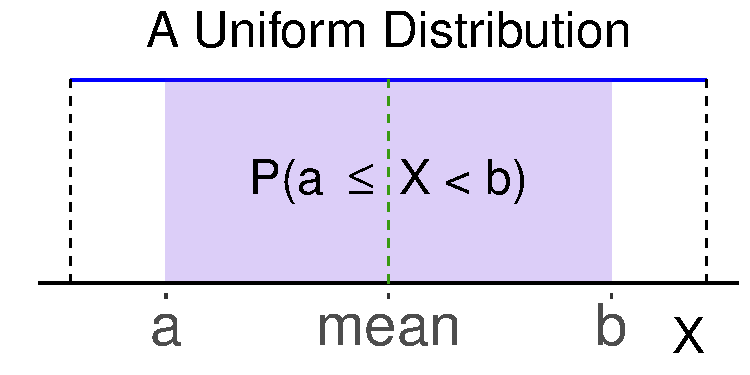
\includegraphics[width=0.8\linewidth]{figure-latex/unnamed-chunk-8-2-1}
        
        \columnbreak

        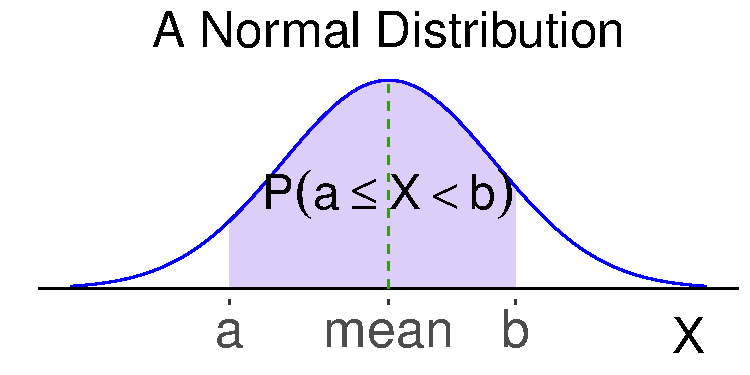
\includegraphics[width=0.8\linewidth]{figure-latex/unnamed-chunk-8-3-1}
      \end{multicols*}
    }}
\end{fullwidth}

\hypertarget{properties-of-probability-distribution-of-a-continuous-random-variable}{%
\subsection{Properties of Probability Distribution of a Continuous
Random
Variable}\label{properties-of-probability-distribution-of-a-continuous-random-variable}}

\begin{itemize}
\item
  The probability density function \(f\) is nonnegative, that is
  \(f(X)\ge 0\).
\item
  The total area under a density curve is 1.
\item
  The cumulative probability \(P(X\le b)\) of a random variable \(X\)
  equals the area under the density curve to the left side of \(b\).
\item
  By the addition rule of probability, we have
    \[P(a\le X\le b)=P(X\le b)-P(X\le a)\]
    \[P(X\ge b)=1-P(X\le b)\]
\item
  As a line segment has no area, we have \(P(X\le a)=P(X< a)\) as well
  as \(P(X\ge b)=P(X>b)\)
\end{itemize}

\begin{example}

Let \(X\) be the amount of time that a commuter must wait for a train.
Suppose \(X\) has a probability density function \[
f(X)=
\begin{cases}
  0.1, & 0\leq X\leq 10\\
  0,   & \text{otherwise}
\end{cases}
\]

What is the probability that the commuter's waiting time is less than 4
minutes?

\end{example}

\vspace*{4\baselineskip}

\hypertarget{normal-distribution}{%
\subsection{Normal Distribution}\label{normal-distribution}}

\begin{itemize}
\item
  A \textbf{normal distribution} has a \textbf{density function}
  \[f(x)=\frac{1}{\sqrt{2\pi \sigma^2}}e^{-\frac{(x-\mu)^2}{2\sigma^2}},\]
  where \(\mu\) is the mean, \(\sigma\) is the standard deviation,
  \(\pi\approx 3.14159\) and \(e\approx 2.71828\). The graph of \(f\) is
  called a \textbf{normal curve}.
\item
  We write \(X\sim N(\mu, \sigma^2)\) for a normal random variable \(X\)
  with the mean \(\mu\) and the standard deviation \(\sigma\).
\item
  A normal distribution has the following properties:

  \begin{itemize}
  \item
    \emph{The mean, median, and mode are equal}.
  \item
    The normal curve is \emph{bell shaped and \textbf{symmetric}} with
    respect to the mean.
  \item
    The \emph{total area} under the curve and above the \(x\)-axis is
    \(1\).
  \item
    The normal curve \emph{approaches, but never touches, the
    \(x\)-axis} as \(x\) goes to \(\pm\infty\).
  \item
    Between \(\mu-\sigma\) and \(\mu+\sigma\), the graph \emph{curves
    downward}. On the left side of \(\mu-\sigma\) or the right side of
    \(\mu+\sigma\), the graph \emph{curves upward}. A point at which the
    curve changes the direction of curving is called an
    \textbf{inflection point}.
  \end{itemize}
\end{itemize}

\begin{fullwidth}
  \colorbox{white}{
    \parbox{\linewidth}{
  \centering
  \textbf{Normal Curves with Different Means and Standard Deviations}

  \begin{multicols*}{2}
    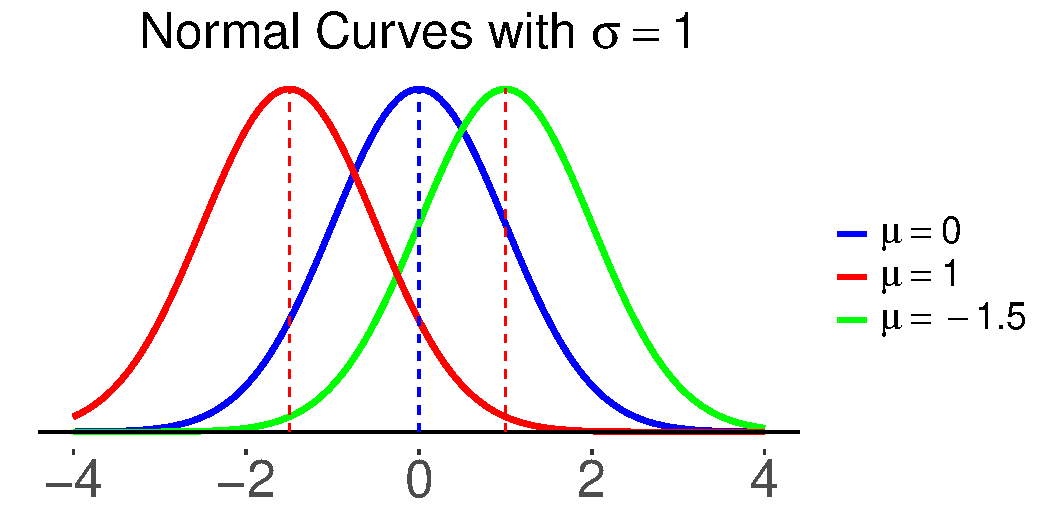
\includegraphics[width=0.8\linewidth]{figure-latex/unnamed-chunk-8-4-1}
    
    \columnbreak

    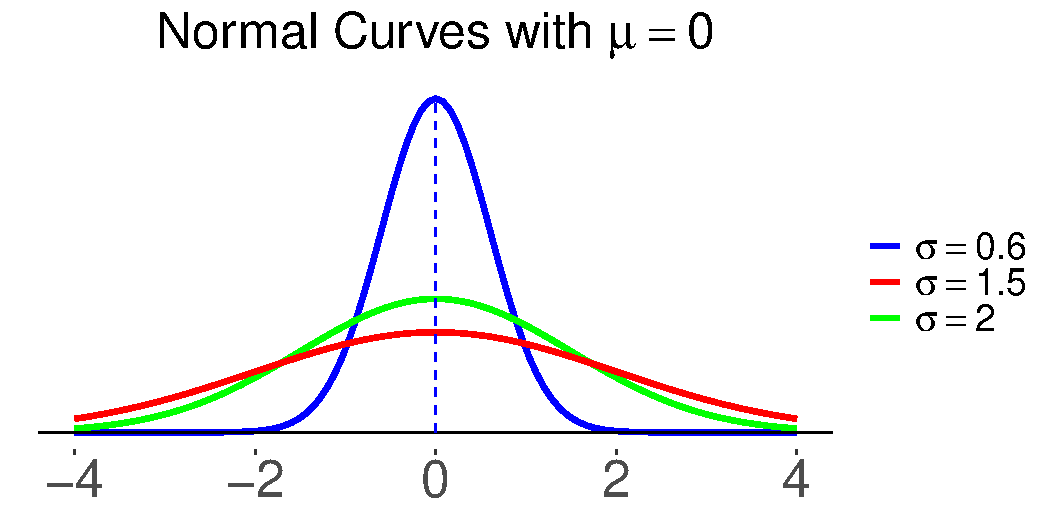
\includegraphics[width=0.8\linewidth]{figure-latex/unnamed-chunk-8-5-1}
  \end{multicols*}
    }}
\end{fullwidth}


\hypertarget{the-empirical-rule-for-normal-distributions}{%
\subsection{The Empirical Rule for Normal
Distributions}\label{the-empirical-rule-for-normal-distributions}}

For any normal distribution, the proportion of data values within 1, 2,
and 3 standard deviations away from the mean are approximately 68.3\%,
95.4\% and 99.7\% respectively.

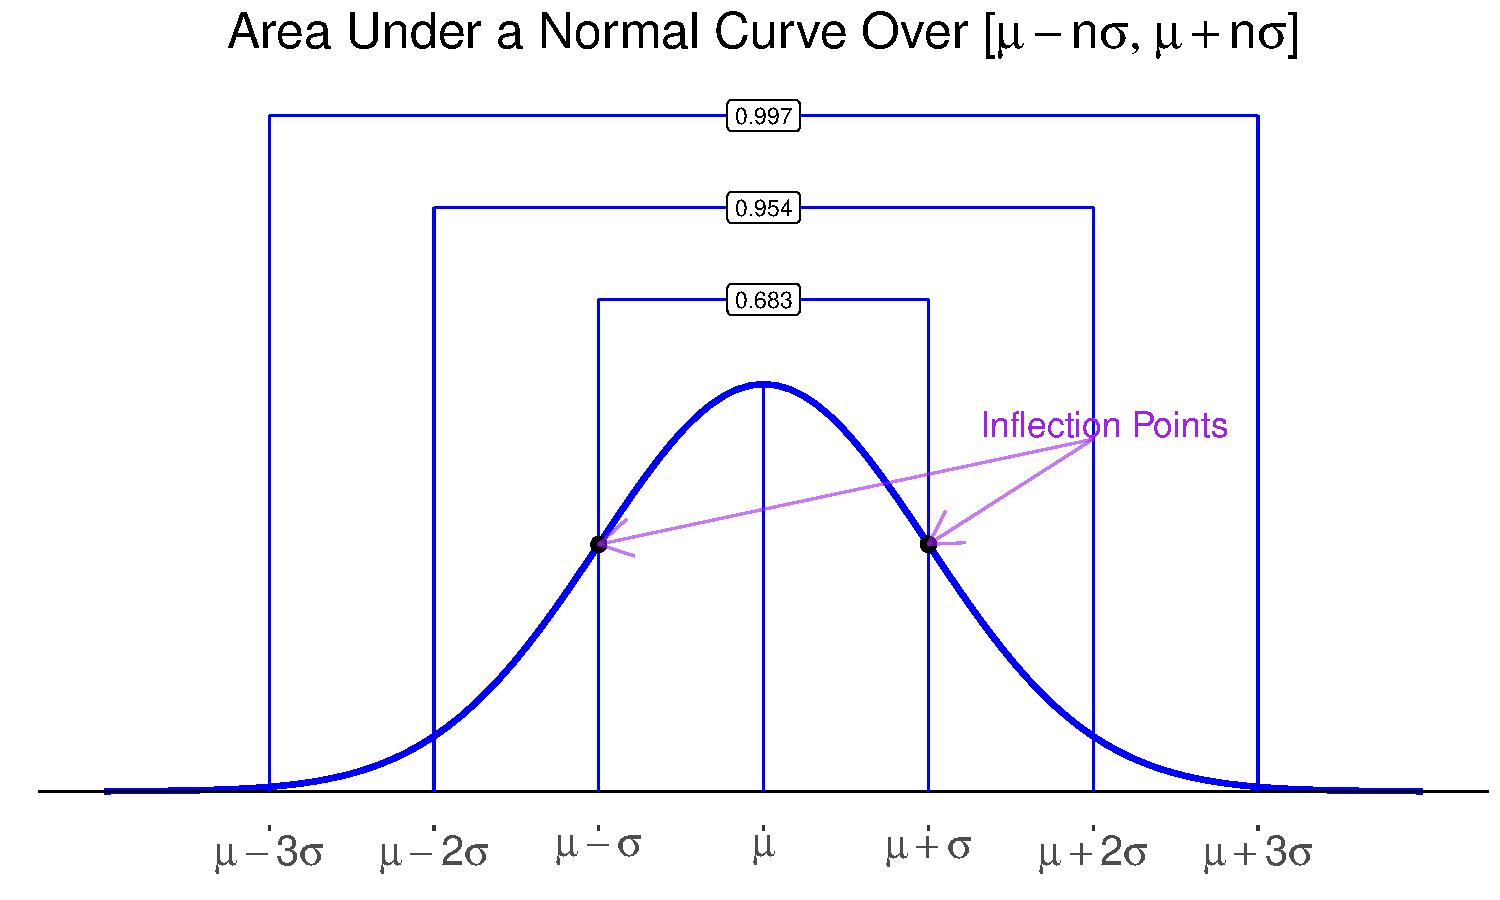
\includegraphics[width=0.8\textwidth]{figure-latex/unnamed-chunk-8-6-1}

\begin{example}

Suppose that foot length of a randomly chosen adult male is a normal
random variable with the mean \(\mu=11\) and the standard deviation
\(\sigma=1.5\).

\begin{enumerate}
\item
  How likely is a male's foot length to be smaller than 9.5 inches
\item
  How likely is a male's foot length to be bigger than 8 inches
\end{enumerate}

\end{example}

\hypertarget{standard-normal-distribution}{%
\subsection{Standard Normal
Distribution}\label{standard-normal-distribution}}

\begin{itemize}
\item
  A normal distribution is called a \textbf{standard normal
  distribution} if the mean is \(\mu=0\) and the standard deviation is
  \(\sigma=1\).
\item
  A random normal variable can be \textbf{standardized} by the following
  formula \(z=\frac{x-\mu}{\sigma}.\) We call the value \(z\) the
  \(Z\)-\textbf{score} of \(x\). In Excel, the \(Z\)-score of \(x\) can
  be calculated using the function \texttt{STANDARDIZE()}.
\item
  Standardization preserves probability:
  \[P(a<X<b)=P\left(\frac{a-\mu}{\sigma}< Z < \frac{b-\mu}{\sigma}\right).\]
\item
  The probability \(P(Z< z)\) of a standard normal random variable \(Z\)
  can be found using the Excel function \texttt{NORM.S,DIST(z,\ TRUE)}.
\item
  The probability \(P(X< x)\) of a normal random variable \(X\) can be
  calculated using the Excel function
  \texttt{NORM.DIST(x,\ mean,\ sd,\ TRUE)}.
\end{itemize}

\begin{example}

Let \(X\) be a norma random variable with the mean \(\mu = 8\) and the
standard deviation \(\sigma=2\).

\begin{enumerate}
\item
  Find the \(Z\)-score for the value \(X=13\).
\item
  Find the \(X\)-value for the \(Z\)-score \(z=-0.6\).
\end{enumerate}

\end{example}

\begin{example}

Let \(Z\) be a standard normal random variable.

\begin{enumerate}
\item
  Find \(P(Z<1.21)\).
\item
  Find \(P(Z\geq 1.21)\).
\item
  Find \(P(0<Z\leq 1.21)\).
\end{enumerate}

\end{example}

\begin{example}

The heights of 25-year-old women in a certain region are approximately
normally distributed with mean 62 inches and standard deviation 4
inches. Find the probability that a randomly selected 25-year-old woman
is more than 67 inches tall.

\end{example}
\vspace*{5\baselineskip}

\hypertarget{cutoff-value-for-a-given-tail-area}{%
\subsection{Cutoff Value for a Given Tail
Area}\label{cutoff-value-for-a-given-tail-area}}

\begin{itemize}
\item
  The \(k\)-th percentile for a random variable \(X\) is the value
  \(x_k\) that cuts off a left tail with the area \(k/100\), that is
  \(P(X<x_k)=\frac{k}{100}\), where \(0\leq k\leq 100\).
\item
  Let \(c\) be a nonnegative number less than or equal to 1. The
  \((100c)\)-th percentile for the standard normal distribution is
  usually denoted as \(-z_c\), that is \(P(Z<-z_c)=c\). By symmetry,
  \(z_c\) is the value such that \(P(Z> z_c)=c\), that is
  \(P(Z<z_c)=1-c\).
\item
  For a normal random variable \(X\) with the mean \(\mu\) and standard
  deviation \(\sigma\), the cutoff value \(x^*\) with a \textbf{tail
  area} \(c\), can be calculated using the standardization formula, that
  is, \[x^*=z^*\cdot \sigma+\mu,\] where \(z^*\) is the cutoff
  \(z\)-score with the tail area \(c\), that is \(z^*=-z_c\) given that
  \(c\) is the left-tail area and \(z^*=z_c\) given that \(c\) is the
  right tail area.
\end{itemize}

\begin{example}

Let \(X\) be the normal random variable with mean \(6\) and standard
deviation \(3\). Suppose the value \(x^*\) cuts off a left-tail area
\(0.05\). Find the value \(x^*\).

\end{example}
\vspace*{4\baselineskip}

\begin{example}

Scores on a standardized college placement examination are normally
distributed with mean 60 and standard deviation 13. Students whose
scores are in the top 5\% will be placed in a Calculus II course. Find
the minimum score needed to be placed in a Calculus II course.

\end{example}
\vspace*{6\baselineskip}

\begin{exercise}

A man arrives at a bus stop at a random time (that is, with no regard for the scheduled service) to catch the next bus. Buses run every  30  minutes without fail, hence the next bus will come any time during the next  30  minutes with evenly distributed probability (a uniform distribution). Find the probability that a bus will come within the next  10  minutes.

\end{exercise}
\vspace*{6\baselineskip}

\begin{exercise}

\begin{enumerate}
\item
  Let \(Z\) be a standard normal random variable. Find the
  probabilities:
  \[\text{1.}\,\, P(Z<1.58)\quad \text{2.}\,\,  P(-0.6<Z<1.67)\quad \text{3.}\,\, P(Z>0.19).\]
\item
  Let \(X\) be a normal random variable with \(\mu=5\) and \(\sigma=2\).
  Find the probabilities:
  \[\text{1.}\,\,  P(-2<X<8)\quad \text{2.}\,\, P(X>-1) \quad \text{3.}\,\, P(X<4).\]
\end{enumerate}

\end{exercise}

\begin{exercise}

The lifetimes of the tread of a certain automobile tire are normally distributed with mean  37,500  miles and standard deviation  4,500  miles. Find the probability that the tread life of a randomly selected tire will be between  30,000  and  40,000  miles.

\end{exercise}
\vspace*{6\baselineskip}

\begin{exercise}

A manufacturer knows that their items have a normally distributed lifespan, with a mean of 9.6 years, and standard deviation of 3 years.

The 4\% of items with the shortest lifespan will last less than how many years?

\end{exercise}
\vspace*{6\baselineskip}

\begin{exercise}

The life of a particular battery is known to follow a normal distribution , with a mean of 1133 hours and a standard deviation of 105 hours.

\begin{enumerate}
  \item 
  What percent of batteries last less than 1033 hours?
  \item 
  The 86 th percentile is represented by what number of hours of battery life? 
  \item
  What is the probability that a randomly selected battery will last more than 1362 hours?
\end{enumerate}

\end{exercise}

\begin{exercise}

Let \(Z\) be a normal random variable with \(\mu=0\) and \(\sigma=1\).
Let \(X\) be a normal random variable with \(\mu=4.3\) and
\(\sigma=1.7\).

Determine the values \(P(Z>1) + P(X<6)\) and explain how do you find the
value.

\end{exercise}
\vspace*{4\baselineskip}

\hypertarget{lab-normal-distributions}{%
\subsection{Lab: Normal Distributions}\label{lab-normal-distributions}}

\begin{itemize}
\item
  Let \(Z\) be a standard normal random variable. In Excel, \(P(Z<z)\)
  is given by \texttt{NORM.S.DIST(z,\ TRUE)}.
\item
  Let \(X\) be a normal random variable with mean \(\mu\) and standard
  deviation \(\sigma\), that is \(X\sim N(\mu, \sigma^2)\). In Excel,
  \(P(X<x)\) is given by \texttt{NORM.DIST(x,\ mean,\ sd,\ TRUE)}.
\item
  When a cumulative probability \(p=P(X<x)\) of a normal random variable
  \(X\) is given, we can find \(x\) using
  \texttt{NORM.INV(p,\ mean,\ sd)}.
\item
  When a cumulative probability \(p=P(Z<z)\) of a standard normal random
  variable \(Z\) is given, we can find \(z\) using
  \texttt{NORM.S.INV(p)}.
\end{itemize}

\begin{exercise}
  Let $Z$ be a standard normal random variable. Find each of the following probabilities. \textbf{Write down the Excel function you used to do the calculation.}

  \begin{enumerate}[itemsep=2.5\baselineskip, after=\vspace*{2\baselineskip}]
    \item $P(Z<0.96)$
    \item $P(Z>-1.43)$
    \item $P(-0.47< Z \le 2.31)$
    \item $P(Z<1.23 \text{~or~} Z>2.13)$
  \end{enumerate}
\end{exercise}

\begin{exercise}
  Let $X$ be a normal random variable with mean  52  and standard deviation  7.
  Find each of the following probabilities. \textbf{Write down the Excel function you used to do the calculation.}

  \begin{enumerate}[itemsep=2.5\baselineskip, after=\vspace*{2\baselineskip}]
    \item $P(X<62)$
    \item $P(X> 35)$
    \item $P(41 < X < 58)$
    \item $P(X<51 \text{~or~} Z>67)$
  \end{enumerate}
\end{exercise}

